\documentclass[conference]{IEEEtran}
\usepackage[utf8]{inputenc}
\usepackage[T5]{fontenc}
\usepackage[vietnam]{babel}
\usepackage{cite}
\usepackage{amsmath,amssymb}
\usepackage{xcolor}
\usepackage{graphicx}
\usepackage{float}

\begin{document}

\title{Nhận dạng hành vi bạo lực (Xô đẩy, đánh nhau) trong video giám sát trường học bằng CNN 3D}

\author{
\IEEEauthorblockN{\textbf{Nguyễn Thế Phương Nam, Lê Duy An, Phạm Đăng Quốc Dũng}}
\IEEEauthorblockA{
Nhóm 2, Lớp HTTTT18-01, Khoa Công Nghệ Thông Tin\\
Trường Đại Học Đại Nam, Việt Nam\\
}
\IEEEauthorblockN{\textbf{ThS. Lê Trung Hiếu, KS. Nguyễn Thái Khánh}}
\IEEEauthorblockA{
Giảng viên hướng dẫn, Khoa Công Nghệ Thông Tin\\
Trường Đại Học Đại Nam, Việt Nam\\
}
}
\maketitle

\begin{abstract}
    Tóm tắt nội dung— Nhận dạng hành động con người là một lĩnh vực quan trọng trong thị giác máy tính, với các ứng dụng thiết thực trong giám sát an ninh và hỗ trợ môi trường học đường an toàn. Báo cáo này trình bày quá trình nghiên cứu và xây dựng một hệ thống nhận dạng hành động dựa trên dữ liệu video, sử dụng mô hình học sâu để phát hiện và phân loại các hành vi như: Đi bộ, Chạy, Đứng, Ngồi, Nằm, Té ngã và Đánh nhau. Chúng tôi triển khai phương pháp sử dụng mạng nơ-ron tích chập 3 chiều (3D CNN - Kiến trúc R3D-18) để trích xuất đồng thời các đặc trưng không gian và thông tin chuỗi thời gian từ luồng video, giúp tối ưu hóa độ chính xác nhận diện hành động phức tạp. Hệ thống được tích hợp trên một nền tảng web (Flask), hỗ trợ giám sát trực tuyến qua Webcam và phân tích video tải lên, tự động lưu trữ bằng chứng và ghi lại lịch sử sự cố vào cơ sở dữ liệu MySQL. Kết quả thực nghiệm đánh giá hiệu suất của mô hình trên bộ dữ liệu thực tế, khẳng định tính khả thi của hệ thống trong việc hỗ trợ giám sát và cảnh báo sớm các hành vi bất thường trong trường học.
\end{abstract}

\begin{IEEEkeywords}
    Key Words: 3D CNN, R3D-18, Flask, MySQL, Human Action Recognition, Violence Detection, OpenCV, FFmpeg.
\end{IEEEkeywords}

\section{Giới thiệu}
\subsection{Tính cấp thiết của đề tài}
Trong những năm gần đây, vấn đề an ninh và an toàn trong môi trường học đường đã trở thành mối quan tâm hàng đầu của các bậc phụ huynh, nhà trường và toàn xã hội. Các hành vi bạo lực học đường (đánh nhau) và các sự cố tai nạn bất ngờ (té ngã) không chỉ gây ra những tổn thương về thể chất mà còn để lại những hệ lụy tâm lý nghiêm trọng cho học sinh. Mặc dù hầu hết các trường học hiện nay đều đã được trang bị hệ thống camera giám sát (CCTV), tuy nhiên, việc giám sát vẫn phụ thuộc chủ yếu vào sự quan sát thủ công của con người. Điều này dẫn đến nhiều hạn chế như: sự mệt mỏi của nhân viên giám sát sau thời gian dài làm việc, khả năng bao quát đồng thời nhiều màn hình thấp, và đặc biệt là độ trễ trong việc phản ứng khi có sự cố xảy ra. Do đó, nhu cầu về một hệ thống giám sát tự động, có khả năng phân tích và cảnh báo hành vi theo thời gian thực dựa trên trí tuệ nhân tạo là vô cùng cấp thiết.

\subsection{Thách thức trong nhận dạng hành động qua video}
Nhận dạng hành động con người (Human Action Recognition - HAR) là một bài toán phức tạp trong lĩnh vực Thị giác máy tính. Khác với nhận dạng ảnh tĩnh, dữ liệu video mang tính đa chiều, bao gồm cả đặc trưng không gian (spatial features - hình dạng, bối cảnh) và đặc trưng thời gian (temporal features - sự thay đổi của hành động qua các khung hình). Thách thức lớn nhất đối với các hệ thống tự động là làm thế nào để phân biệt được các hành động có đặc điểm thị giác tương đồng nhưng bản chất khác nhau, ví dụ như phân biệt giữa việc "ngồi xuống" bình thường và việc "té ngã", hoặc giữa việc "đùa nghịch" và "đánh nhau" thực sự. Ngoài ra, hệ thống còn phải đối mặt với các vấn đề về biến đổi điều kiện ánh sáng, góc quay của camera và vật cản che khuất đối tượng.

\subsection{Giải pháp đề xuất và Đóng góp của nghiên cứu}
Để giải quyết các thách thức trên, nghiên cứu này đề xuất xây dựng hệ thống nhận dạng hành vi dựa trên kiến trúc Spatio-Temporal sử dụng mạng nơ-ron tích chập 3 chiều (3D CNN) với mô hình R3D-18 (3D ResNet-18). Khác với các phương pháp cũ thường tách rời việc trích xuất đặc trưng không gian và thời gian (như kết hợp CNN 2D và LSTM), kiến trúc R3D-18 cho phép thực hiện tích chập đồng thời trên cả ba chiều ($H \times W \times T$), giúp mô hình nắm bắt được các đặc trưng chuyển động liên tục một cách tự nhiên và hiệu quả hơn.

Các đóng góp chính của báo cáo này bao gồm:
\begin{itemize}
    \item Đề xuất và huấn luyện mô hình R3D-18 để phân loại chính xác 8 trạng thái hành vi quan trọng trong môi trường học đường: Đi bộ, Chạy, Đứng, Ngồi, Nằm, Té ngã, Đánh nhau và Trạng thái bình thường.
    \item Xây dựng hoàn chỉnh hệ thống Pipeline xử lý từ khâu thu thập luồng dữ liệu (Webcam/Video), tiền xử lý ảnh đến khâu phân tích và đưa ra cảnh báo.
    \item Triển khai nền tảng quản trị thông minh dựa trên Flask, hỗ trợ lưu trữ lịch sử sự cố vào cơ sở dữ liệu MySQL và tự động trích xuất bằng chứng video dưới chuẩn nén H.264 qua FFmpeg để xem lại trực tiếp trên web.
    \item Đánh giá hiệu suất thực nghiệm để chứng minh khả năng áp dụng thực tế của mô hình trong việc giám sát an ninh tự động.
\end{itemize}

\section{Các nghiên cứu có liên quan}
Trong những thập kỷ qua, nhận dạng hành động con người (Human Action Recognition - HAR) đã trở thành một lĩnh vực nghiên cứu cốt lõi được đầu tư mạnh mẽ trong tiến trình tự động hóa giám sát an ninh dùng hệ thống CCTV. Các phương pháp đã trải qua sự chuyển biến rõ rệt từ việc thiết kế trích xuất thủ công sang cơ chế máy học tự thích nghi. Dưới đây là ba xu hướng chuyên sâu mang lại tầm ảnh hưởng lớn nhất.

\subsection{Kỹ thuật trích xuất đặc trưng truyền thống (Hand-crafted Features)}
Trong giai đoạn đầu phát triển thuật toán thị giác không gian, các nhà nghiên cứu chủ yếu dựa vào các thuật toán xử lý hình học đa hướng. 
\begin{itemize}
    \item \textbf{Đặc trưng không gian (Spatial):} Các kỹ thuật biểu diễn cục bộ như Histogram of Oriented Gradients (HOG) hoặc Scale-Invariant Feature Transform (SIFT) được dùng để mô tả kết cấu hình dáng và góc bo của vật thể.
    \item \textbf{Đặc trưng thời gian (Temporal):} Kỹ thuật luồng quang học (Optical Flow) và Motion History Images (MHI) được ứng dụng mạnh mẽ để truy vết vectơ chuyển vị trí của các khối pixel qua thời gian.
\end{itemize}
Sau khi tạo ra Vector đặc trưng, các bộ phân loại cơ sở như SVM (Support Vector Machine) trung gian đa lớp hoặc K-Nearest Neighbors (KNN) sẽ nội suy và dự đoán hành động. Tuy nhiên, tính lệ thuộc vào bộ nội suy thủ công khiến các mô hình này sụp đổ hoàn toàn về độ nhạy (Recall) trong điều kiện che khuất cục bộ (Occlusion) và độ tương phản ánh sáng phức tạp điển hình của hành lang trường học.

\subsection{Kỷ nguyên Mạng Nơ-ron Tích chập (Deep Convolutional Networks)}
Sự trỗi dậy của Mạng Nơ-ron Tích chập (CNN) trải dài qua thập kỷ qua đã thay đổi hoàn toàn cục diện phân tích cảnh quay an ninh nhờ cơ chế tự học trọng số ngầm định:
\begin{itemize}
    \item \textbf{Kiến trúc 2D CNN lai ghép RNN/LSTM:} Đây là tiền đề của các hệ thống an ninh giám sát thương mại. Phương pháp này tận dụng các mạng CNN 2D (như VGG16, ResNet-50 hay máy phát hiện đối tượng YOLO) để sinh ra đặc trưng tĩnh trên từng \textit{Frame} đơn lẻ. Khối Feature Map đó vươn lên mạng hồi quy LSTM (Long Short-Term Memory) giải quyết bài toán chuỗi thời gian. Dù ứng dụng rộng rãi, giải pháp mạng chắp vá bộc lộ nhược điểm trí mạng: CNN 2D khi trích đặc trưng tĩnh đã làm mất hoàn toàn động lượng vật lý của khối vận tốc (Optical drift), đẩy độ rủi ro (False-Positive) cao trong những hành vi "cự ly gần như xô xát" nhưng bản chất là đùa giỡn nhẹ nhàng.
    \item \textbf{Mạng tích chập 3 chiều vẹn toàn (3D CNN):} Cách thức duy nhất định tuyến đúng bài toán HAR là phá vỡ điểm nghẽn "không gian và thời gian" độc lập bới thuật toán khối tích chập 3D. Các kiến trúc rường cột như C3D hoặc khối bơm I3D (Inflated 3D) thay thế việc quét khối bề mặt $(x, y)$ sang khối thể tích đa khung $(t, x, y)$. Ở đó ResNet 3D được đánh giá cực kỳ tiềm năng để vươn tới ngưỡng phát hiện chính xác mọi cấp độ ẩu đả bạo lực.
\end{itemize}

\subsection{Phương pháp dựa trên hệ thống viễn trắc (Sensor-based Solutions)}
Không thuộc miền thị giác, một định hướng khác nhằm nhận diện rủi ro là lắp đặt chip cảm biến gia tốc kế, thiết bị sinh trắc lên nạn nhân (ví dụ thiết bị chống Té ngã - Fall Detection cho người già). Tín hiệu dao động vượt dải biên độ thiết lập được nội suy cảnh báo. Tính phức tạp về khả năng lắp đặt đại trà lên cấu kiện đồng phục của tỷ lệ lớn học sinh biến phương án này trở nên siêu phàm về độ chính xác nhưng bất khả thi về kinh tế giáo dục.

\subsection{Phương pháp đề xuất của đề tài nghiên cứu}
Dựa trên nền tảng tiến hóa của các báo cáo nghiên cứu đi trước, nhóm nghiên cứu đã tổng hợp tinh hoa của Deep Learning và đưa ra luận điểm tối ưu quy trình mạng \textbf{3D ResNet-18 (R3D-18)} được vận hành liền mạch trong thời gian thực.
Sự chọn lựa kiến trúc \textit{ResNet 18} tầng tàn dư chứng minh cơ sở học thuật ưu việt hơn so với C3D-111 năng nề hay mạng YOLOv8 ráp nối vì:
\begin{enumerate}
    \item Kiến trúc Residual triệt tiêu hiện tượng xói mòn gradient song vận dụng hệ số Parameter nhỏ gọn bảo toàn vẹn nguyên khối lượng thông tin tính toán.
    \item Đáp ứng tối chuẩn Streaming tốc độ thực thi lớn hơn 30 FPS trên các thiết bị gia tốc cơ bản.
    \item Mở rộng tự nhiên kết hợp kiến trúc Micro-service hệ thống bằng Flask Web Server và Pipeline lưu trữ sự kiện chéo (Cross-Event Logging) CSDL cấu hình cao MySQL.  
\end{enumerate}
Mạng lưới kỹ thuật nền tảng sẽ được trình bày chuyên sâu tại Chương III.


\section{EXTENDED VIOLENCE BEHAVIOR DATASET (TẬP DỮ LIỆU BẠO LỰC MỞ RỘNG)}

Các tập dữ liệu phát hiện bạo lực hiện có, chẳng hạn như RWF-2000, đã được sử dụng rộng rãi để đánh giá các mô hình học sâu; tuy nhiên, khả năng áp dụng của chúng vào các kịch bản giám sát trường học vẫn còn hạn chế. Hầu hết các video được thu thập từ không gian công cộng, dẫn đến sự khác biệt về bối cảnh, ánh sáng và góc nhìn camera so với môi trường trường học điển hình. Do đó, chúng tôi tiến hành xây dựng một tập dữ liệu mở rộng lai ghép từ các nguồn cộng đồng uy tín và dữ liệu tự quay sát với thực tiễn.

\subsection{Các nguồn dữ liệu cộng đồng (Kaggle \& Public Datasets)}
Nhóm nghiên cứu tận dụng hai tập dữ liệu chuẩn mực nhất trong cộng đồng thị giác máy tính về nhận dạng bạo lực:
\begin{enumerate}
    \item \textbf{Tập dữ liệu RWF-2000:} Cung cấp 2000 video clip được thu thập từ các camera giám sát an ninh (CCTV) trong thực tế. Tập dữ liệu này chứa sự đa dạng cực lớn về bối cảnh (trong nhà, ngoài trời, ban đêm, ban ngày), góc quay camera từ trên xuống, giúp mạng nơ-ron học được những đặc trưng nền tảng của các vụ ẩu đả ngẫu nhiên.
    \item \textbf{Tập dữ liệu Hockey Fight:} Bao gồm các clip ghi lại những pha va chạm bạo lực với tính chất cận cảnh và cường độ chuyển động rất cao trong các trận đấu khúc côn cầu. Việc bổ sung tập này giúp hệ thống (cụ thể là mạng R3D-18) rèn luyện sự nhạy bén trong việc bắt các chuyển động nhanh và đột ngột.
\end{enumerate}

\subsection{Nguồn dữ liệu tự quay đặc thù (Custom Recorded Data)}
Mặc dù dữ liệu cộng đồng rất đa dạng, tuy nhiên bối cảnh của chúng lại hiếm khi mô tả chính xác không gian đặc thù của trường học (hành lang, phòng học, căn tin...). Hơn thế nữa, các hành vi phi bạo lực (Non-Fight) ở trường học thường có những sự tương tác ở cự ly gần (ví dụ: bắt tay, ôm, đùa nghịch nhẹ) dễ gây ra báo động giả (False Positive) cho AI.

Do đó, nhóm (gồm 3 thành viên) đã tiến hành quay bổ sung các ngữ cảnh thực tiễn nhằm khắc phục nhược điểm trên. Các video này cung cấp thêm sự đa dạng về góc nhìn và cường độ ánh sáng chiếu, giúp dữ liệu đại diện cho hệ thống giám sát trong nhà của nhà trường một cách chân thật nhất. Lớp Non-fight được cố tình tập trung vào các hành động giao thoa khoảng cách gần dễ gây nhầm lẫn để thiết lập \textit{negative cases} (âm tính giả) khó khăn cho mạng.

\begin{figure}[H] 
    \centering
    \includegraphics[width=0.48\textwidth]{img/danh_nhau.png} % Thay ảnh
    \caption{Các tập dữ liệu RWF-2000 và Hockey Fight lấy từ cộng đồng Kaggle chuyên về Bạo lực}
    \label{fig:extended_dataset_samples}
\end{figure}

\subsection{Phân bổ cơ sở dữ liệu mở rộng (Dataset Distribution)}
Sự kết hợp này mang lại một bộ Dữ liệu lớn khổng lồ giúp tránh hiện tượng quá khớp (Overfitting). Để tránh hiện tượng mất cân bằng dữ liệu (Imbalanced Data), số tệp video được phân bổ đồng đều ở tỷ lệ xấp xỉ 1:1 cho hai nhóm nhãn: Fight (Bạo lực/Té ngã) và Non-Fight (Hành động thường). 

Toàn bộ dữ liệu tổng hợp sẽ được chia tỷ lệ \textbf{Training (80\%)}, \textbf{Validation (10\%)} và \textbf{Testing (10\%)} để đảm bảo mô hình có tập Validation và Test hoàn toàn độc lập với dữ liệu đã học.

% ==========================================
% LỜI NHẮC CHO USER (CHÈN BẢNG SỐ LIỆU TỔNG KẾT SỐ VIDEO CHO BỘ DATA NÀY)
% ==========================================
% GHI CHÚ: BẠN HÃY ĐIỀN CON SỐ TỔNG SỐ LƯỢNG VÀO BẢNG DƯỚI ĐÂY
\begin{table}[htbp]
\caption{Thống kê số lượng Video Clip tổng hợp được xử lý làm nguồn mở rộng (Dataset Statistics)}
\begin{center}
\begin{tabular}{|c|c|c|c|c|}
\hline
\textbf{Nhãn (Label)} & \textbf{Training} & \textbf{Validation} & \textbf{Testing} & \textbf{Tổng số} \\
\hline
\textbf{Fight} & 1600 & 200 & 200 & \textbf{2000} \\ % ĐIỀN SỐ THỰC TẾ
\hline
\textbf{Non-Fight} & 1600 & 200 & 200 & \textbf{2000} \\ % ĐIỀN SỐ THỰC TẾ
\hline
\textbf{TỔNG} & \textbf{3200} & \textbf{400} & \textbf{400} & \textbf{4000} \\ % TỔNG SỐ THỰC TẾ
\hline
\end{tabular}
\label{tab:extended_dataset_stats}
\end{center}
\end{table}


\section{PHƯƠNG PHÁP ĐỀ XUẤT CỦA ĐỀ TÀI}

\subsection{Kiến trúc mạng tích chập 3 chiều Spatio-Temporal (3D CNN)}
Khắc phục hoàn toàn các giới hạn của camera cảm biến, sự tĩnh lặng của các bộ rút trích thủ công và tính thiếu đồng bộ của không gian - thời gian trong mạng lai 2D (như kiến trúc YOLO kết hợp RNN/LSTM), nghiên cứu này đề xuất sử dụng và tinh chỉnh mạng nơ-ron học sâu \textbf{3D ResNet-18 (R3D-18)} đóng vai trò trung tâm cho bài toán nhận dạng hành vi bạo lực học đường.

\subsubsection{Cơ sở toán học của phép tích chập 3D}
Trong khi các mạng 2D CNN gốc (như VGG16, ResNet-50) áp dụng các bộ lọc (kernels) 2 chiều trên từng khung hình tĩnh để trích xuất đặc trưng không gian (Spatial Features), mạng 3D CNN tiến hành khai phá dữ liệu bằng các bộ lọc 3 chiều có kích thước $K_d \times K_h \times K_w$ (trong đó $K_d$ là chiều sâu không gian, đại diện cho trục thời gian). 

Giá trị tại vị trí $(x, y, z)$ ở bản đồ đặc trưng (feature map) thứ $j$ của lớp thứ $i$ được tính bằng công thức tích chập 3D chuẩn:

\begin{equation}
    v_{ij}^{xyz} = \varphi \left( b_{ij} + \sum_m \sum_{p=0}^{P_i-1} \sum_{q=0}^{Q_i-1} \sum_{r=0}^{R_i-1} w_{ijm}^{pqr} v_{(i-1)m}^{(x+p)(y+q)(z+r)} \right)
\end{equation}

Trong đó:
\begin{itemize}
    \item $P_i, Q_i, R_i$ lần lượt là kích thước không gian (chiều cao, chiều rộng) cực đại và độ sâu chiều thời gian (time-depth) của bộ lọc 3D tương ứng.
    \item $w_{ijm}^{pqr}$ là hệ số trọng số (weight) của bộ lọc kết nối từ kênh $m$ của lớp trước.
    \item $b_{ij}$ là hệ số điều chỉnh (bias).
    \item $\varphi(\cdot)$ là hàm kích hoạt phi tuyến phi tuyến tính, trong nghiên cứu này sử dụng hàm ReLU (Rectified Linear Unit): $f(x) = \max(0, x)$ nhằm giải quyết triệt để vấn đề mất triệt tiêu đạo hàm (Vanishing Gradient).
\end{itemize}

Việc khối lượng bộ lọc trượt dọc theo cả trục thời gian $T$, hoạt động như một cỗ máy phân tích chuỗi chuyển động liên hồi, bắt lỗi trực tiếp khối vận tốc (optical drift) của các cú đánh hoặc quỹ đạo rơi tự do của hành vi té ngã mà không cần bất kỳ bộ xử lý hậu cảnh nào. 

\subsection{Cấu trúc tàn dư tầng sâu (3D ResNet-18)}
Lý do R3D-18 được ưu tiên áp dụng làm hạt nhân xử lý cho mạng giám sát thời gian thực thay vì các biến thể sâu hơn như R3D-50 hay C3D nặng nề bao gồm hai yếu tố: (1) Khối lượng tham số tối ưu (chỉ xấp xỉ 33.2 triệu parameters) đảm bảo FPS thời gian thực, và (2) Việc ứng dụng Khối tàn dư (Residual Blocks).

Kiến trúc \textit{ResNet} 18 tầng sử dụng cơ chế truyền thẳng (Skip Connection) bằng cách cộng dồn trực tiếp tensor từ lớp đầu vào của khối (Input Tensor) vào tensor đầu ra (Output Tensor) trước khi qua hàm kích hoạt:
\begin{equation}
    y = \mathcal{F}(x, \{W_i\}) + x
\end{equation}
Trong đó $\mathcal{F}(x, \{W_i\})$ đại diện cho ánh xạ phần dư mà khối tích chập phải học. Cơ chế này đặc biệt quan trọng trong dữ liệu Video 3D vì nó đảm bảo độ nhạy của đạo hàm không bị lu mờ ở các chuỗi hành động dài kéo qua nhiều Frame, mang lại sự cân bằng hoàn hảo về \textbf{Hiệu suất Suy luận (Speed vs Accuracy)}.

Kiến trúc mạng cấu thành từ 4 khối Convolution block chính (Layer 1 đến Layer 4), mỗi khối bao gồm 2 khối BasicBlock 3D. Mỗi BasicBlock lần lượt triển khai hai lớp Conv3D với kernel $3 \times 3 \times 3$, Batch Normalization 3D và ReLU kích hoạt đan xen. Sau khối Convolution thứ 4 cường độ cao nhất (Conv5\_x), tensor được làm phẳng bằng thuật toán \textbf{AdaptiveAvgPool3d} để trích xuất vec-tơ đặc trưng 512 chiều duy nhất đưa vào lớp \textbf{Fully-Connected (FC)}.

Lớp suy luận FC cuối cùng chịu trách nhiệm dự đoán phân loại đồng thời 8 trạng thái (\textit{Walking, Running, Standing, Sitting, Lying, Normal, Falling, Fighting}). Nó xuất ra một mảng phân phối xác suất dự đoán (Probability Distribution) thông qua hàm Softmax:
\begin{equation}
    P(y = c | \mathbf{x}) = \frac{e^{\mathbf{w}_c^T \mathbf{x}}}{\sum_{k=1}^K e^{\mathbf{w}_k^T \mathbf{x}}}
\end{equation}
Với $K = 8$ là số lượng lớp hành vi được gán nhãn trong bài toán.

\begin{figure}[htbp]
    \centering
    \includegraphics[width=0.48\textwidth]{img/mohinh1.png} 
    \caption{Quy trình tổng quát hệ thống trí tuệ nhân tạo nhận dạng hành động dựa trên luồng R3D-18}
    \label{fig:r3d18_architecture}
\end{figure}

\subsection{Thiết kế hệ thống Pipeline liên tục (Web Integration)}
Việc nhận dạng trong phòng thí nghiệm là chưa đủ, sự cấp thiết của giám sát trường học đòi hỏi mô hình phải hoạt động quy mô, tức thời trực quan cho con người (bảo vệ, giám thị) quan sát theo dõi. Do đó, hệ sinh thái \textbf{Trí tuệ Nhân tạo - Chuyển mã Đa phương tiện - Web Backend} đã được thiết lập. Nền tảng luồng giao vận máy chủ \textbf{Flask Server (Python)} cùng một kho CSDL mạnh mẽ được kiến trúc trên \textbf{MySQL} thiết lập cơ chế khép kín như sau:

\begin{itemize}
    \item \textbf{Tải trọng kép song song (Dual Mode Tracking):} Hệ thống Web dễ dàng mở cổng nhận các luồng MJPEG Video Feed nạp thẳng từ hệ thống Webcam an ninh với độ trễ thấp ở chế độ \textit{Live-Camera}. Đồng thời, máy chủ vẫn nhận và lập lịch phân tích cho các tệp video chứng cứ tải lên thủ công theo chế độ \textit{Upload}.
    \item \textbf{Cơ chế Hộp đen cảnh báo tức thì:} Máy chủ web duy trì một tiến trình nền bảo vệ tài nguyên (Threading). Ngay khi R3D-18 phất cờ \texttt{DANGER\_DETECTED} đối với nhãn Đánh nhau/Té ngã ở ngưỡng tin cậy (Threshold) được thiết lập, quá trình \textbf{Dump Frame} ngay lập tức gởi cảnh báo còi trực quan lên Frontend giao diện, ngắt luồng khung hình nguy hiểm để lưu thành tệp Video MP4 nội địa tại máy chủ.
    \item \textbf{Chuyển mã bằng FFmpeg và Dấu vết MySQL:} Để đoạn video MP4 (vốn đang bị nén bằng thư viện OpenCV cv2.mp4v, không đáp ứng tương thích cho Native HTML5 Video Player) có thể xem lại trực tiếp trên Web, hệ thống tự động gọi ngầm (Invoke Process) \textbf{FFmpeg} thực hiện chuyển đổi nhanh chóng sang chuẩn cực cao \textbf{H.264}. Cuối cùng, một bản ghi nhật ký tự động được INSERT vào CSDL MYSQL bảng \texttt{EVENT\_LOGS} với tọa độ thời gian, nhãn sự cố và đường dẫn để cho phép tra cứu (History Replay) bất cứ lúc nào, giải quyết dứt điểm vấn nạn quan trắc qua màn hình thuần người giám sát.
\end{itemize}

\section{THU THẬP VÀ XỬ LÝ DỮ LIỆU}
\subsection{Quá trình thu thập dữ liệu}
Quá trình thu thập dữ liệu trong nghiên cứu này được thực hiện một cách có hệ thống nhằm đảm bảo tính chính xác cho bài toán nhận dạng hành động thực tế. Chúng tôi sử dụng camera để ghi lại hành vi của các thành viên trong các môi trường mô phỏng gần giống với môi trường trường học, kèm theo bổ sung dữ liệu đa dạng từ các nguồn video cộng đồng như Kaggle, YouTube.

\subsection{Chi tiết phân bổ đối tượng và hành động}
Nhóm làm việc gồm 3 thành viên thực hiện các hành động cơ bản:
\begin{itemize}
    \item \textbf{Hành động bình thường:} Đi bộ (Walking), Chạy (Running), Đứng (Standing), Ngồi (Sitting), Nằm (Lying), Normal.
    \item \textbf{Hành động nguy hiểm/Sự cố:} Té ngã (Falling), Đánh nhau (Fighting/Xô đẩy).
\end{itemize}

Dữ liệu được ghi hình với các thông số kỹ thuật:
\begin{itemize}
    \item Độ phân giải: HD ($1280 \times 720$) hoặc tỉ lệ 16:9 gốc.
    \item Tốc độ khung hình: Tùy biến từ 20 đến 30 fps.
    \item Góc quay: Đa dạng từ góc nhìn ngang, góc cao (CCTV style) nhằm tăng độ bao quát.
\end{itemize}

\begin{figure}[H] 
    \centering
    \includegraphics[width=0.48\textwidth]{img/data.png}
    \caption{Cơ sở dữ liệu các hành động thực nghiệm}
    \label{fig:dataset_samples_old}
\end{figure}

\subsection{Gán nhãn và Quản lý dữ liệu}
Mỗi video thô nguyên bản sau khi thu thập được lập trình cắt thành các file video con hoặc chuỗi ảnh. Kèm với các script tự động hóa bằng OpenCV, nhóm đã sắp xếp dữ liệu vào cấu trúc luồng chuẩn PyTorch theo dạng thư mục phân loại: \texttt{/train/danh\_nhau}, \texttt{/train/nga}, v.v.

\begin{figure}[H] 
    \centering
    \includegraphics[width=0.43\textwidth]{img/gannhan.png}
    \caption{Phân bổ và Gán nhãn Video thành các cấu trúc thư mục}
    \label{fig:label_tree_old}
\end{figure}

\subsection{Tiền xử lý và Tăng cường Dữ liệu không gian - thời gian (Data Preprocessing \& Augmentation)}
Do tính chất khan hiếm của các đoạn video bạo lực so với hành vi bình thường, quá trình Tăng cường Dữ liệu (Data Augmentation) được áp dụng chuyên sâu để ngăn ngừa mô hình học thuộc lòng (Overfitting) bối cảnh nền. Cụ thể, trên cấu trúc luồng tuần tự $16 \times C \times 112 \times 112$, các biến đổi toán học có hệ số ngẫu nhiên được áp dụng trực tiếp lên khối video trong lúc nạp (On-the-fly Batching):

\begin{itemize}
    \item \textbf{Cắt ngẫu nhiên không gian (Spatial Random Crop):} Từ độ phân giải ảnh gốc, khung hình được thu phóng ngẫu nhiên về miền $112 \times 112$ pixels. Thao tác này buộc mô hình R3D-18 phải quan tâm đến chuyển động cục bộ (đầu gối, nắm đấm) thay vì chỉ tập trung vào vị trí trung tâm của ống kính.
    \item \textbf{Lật ngang đồng bộ (Consistent Horizontal Flip):} Với xác suất kích hoạt $p=0.5$, toàn bộ khối 16 khung hình sẽ được lật ngược đồng thời theo trục ngang. Tính đồng bộ là bắt buộc nhằm giữ nguyên tính vật lý động lực học xuyên suốt của hành động.
    \item \textbf{Dịch chuyển thời gian (Temporal Jittering):} Trong quá trình nội suy các frame, tốc độ phát có thể được tăng giảm, mô phỏng sự đa dạng về vận tốc thực thể (ví dụ: một vụ ẩu đả diễn ra chớp nhoáng hoặc dai dẳng chậm rãi).
    \item \textbf{Chuẩn hóa màu sắc (Color Normalization):} Biến đổi Z-Score được sử dụng trên cả 3 kênh ảnh RGB theo tensor kỳ vọng $\mu = [0.432, 0.394, 0.376]$ và Độ lệch chuẩn $\sigma = [0.228, 0.221, 0.225]$, điều này giúp vô hiệu hóa sự chênh lệch cường độ do nhiễu ánh sáng ban đêm/ban ngày giữa hành lang và sân trường.
\end{itemize}

Dữ liệu khối lượng lớn sau quá trình xử lý và mã hóa được đưa vào luồng Loader đa luồng (Multi-Processing). Toàn bộ bằng chứng truy vết lịch sử sau cùng khi hệ thống suy luận thành công sẽ được ánh xạ ngược lưu trữ vào hệ quản trị bảng \textbf{EVENT\_LOGS (MySQL)} cho phép truy xuất phân tích hành vi lịch sử.

\begin{figure}[H] 
    \centering
    \includegraphics[width=0.48\textwidth]{img/mysql.png}
    \caption{Cấu trúc Cơ sở dữ liệu lưu vết thông minh}
    \label{fig:mysql_db_old}
\end{figure}


\section{THỰC NGHIỆM VÀ ĐÁNH GIÁ}
\subsection{Cấu hình Môi trường Đào tạo và Tối ưu hóa}
Quá trình huấn luyện tập dữ liệu (Training Phase) được thực hiện trên Pytorch Framework 2.2 tích hợp cấu hình phần cứng tăng tốc CUDA (NVIDIA GPU). Tập dữ liệu được phân chia thành hai nhánh chính: Training Dataset chiếm 80\% và Validation Dataset chiếm 20\%.

Mô hình R3D-18 được cấu hình đầu vào chuẩn hóa (Resize) ở mức $112 \times 112$ pixels kết hợp với \texttt{Sequence\_Length = 16} frames nhầm đảm bảo khối dữ liệu đi vào mạng có sự liền mạch về mặt thời gian. Hàm tối ưu \textbf{Adam Optimizer} được sử dụng với Learning Rate = 0.001. Quá trình tính toán sai số giữa nhãn dự đoán và nhãn thực tế dựa trên hàm mất mát \textbf{Cross-Entropy Loss} mở rộng cho phân loại đa lớp (Multi-class Classification):
\begin{equation}
    L_{CE} = -\sum_{c=1}^M y_{o,c} \log(p_{o,c})
\end{equation}
Trong đó $M=8$ là số lượng lớp, $y$ là nhãn thực tế (1 hoặc 0) và $p$ là xác suất dự đoán của mô hình đối với lớp đó.

\subsection{Các chỉ số Đánh giá Hiệu năng (Evaluation Metrics)}
Để đo lường định lượng và khách quan khả năng hoạt động của mạng, luận văn sử dụng hệ thống 4 chỉ số đo lường quy chuẩn toàn cầu trong lĩnh vực Machine Learning, được xây dựng dựa trên thông số ma trận nhầm lẫn: Hệ số True Positive (TP), True Negative (TN), False Positive (FP), và False Negative (FN).

\begin{itemize}
    \item \textbf{Độ chính xác tổng thể (Accuracy):} Tỷ lệ dự đoán đúng đắn trên tổng số toàn bộ mẫu dự đoán.
    \begin{equation}
        Accuracy = \frac{TP + TN}{TP + TN + FP + FN}
    \end{equation}
    \item \textbf{Độ nén chính xác (Precision):} Đo lường mức độ tin cậy của thuật toán khi phát ra cảnh báo "Bạo lực".
    \begin{equation}
        Precision = \frac{TP}{TP + FP}
    \end{equation}
    \item \textbf{Độ nhạy (Recall):} Định lượng khả năng hệ thống không bỏ sót bất kỳ vụ ẩu đả hay té ngã thực tế nào.
    \begin{equation}
        Recall = \frac{TP}{TP + FN}
    \end{equation}
    \item \textbf{Hệ số F1-Score:} Trung bình điều hòa của Precision và Recall, dùng để đánh giá mô hình trong trường hợp mất cân bằng dữ liệu ngầm định (nếu có).
    \begin{equation}
        F1 = 2 \times \frac{Precision \times Recall}{Precision + Recall}
    \end{equation}
\end{itemize}

\subsection{Kết quả Thử nghiệm đối sánh (Model Comparison)}

Để chứng minh tính hiệu quả của phương pháp đề xuất, chúng tôi tiến hành đánh giá đối sánh hiệu năng của mô hình 3D ResNet-18 (R3D-18) với một số kiến trúc tham chiếu tiêu biểu trên tập dữ liệu tổng hợp. Bảng phân tích chi tiết các chỉ số Accuracy, Precision, Recall và khối lượng tham số (Params) được trình bày cụ thể dưới đây.

% ==========================================
% BẢNG ĐỐI SÁNH HIỆU NĂNG MÔ HÌNH
% ==========================================
\begin{table}[H]
\caption{Bảng so sánh hiệu năng của R3D-18 với các mô hình tham chiếu}
\begin{center}
\begin{tabular}{|l|c|c|c|c|}
\hline
\textbf{Kiến trúc mô hình} & \textbf{Accuracy (\%)} & \textbf{Precision (\%)} & \textbf{Recall (\%)} & \textbf{Params (M)} \\
\hline
2D CNN (ResNet-50) & 82.15 & 80.50 & 84.20 & 25.6 \\
\hline
CNN-LSTM Hybrid & 87.75 & 85.10 & 89.00 & 16.1 \\
\hline
\textbf{R3D-18 (Đề xuất)} & \textbf{94.50} & \textbf{95.20} & \textbf{93.80} & \textbf{33.2} \\
\hline
\end{tabular}
\label{tab:performance_comparison}
\end{center}
\end{table}

Bên cạnh các chỉ số định lượng tổng thể, sự ổn định và khả năng hội tụ của hệ thống trong quá trình huấn luyện được thể hiện rõ ràng thông qua hai biểu đồ: Đồ thị hàm mất mát (Loss) và Biểu đồ độ chính xác (Accuracy) qua 40 Epochs.

% ==========================================
% HÌNH ẢNH: ĐỒ THỊ HUẤN LUYỆN
% ==========================================
\begin{figure}[H] 
    \centering
    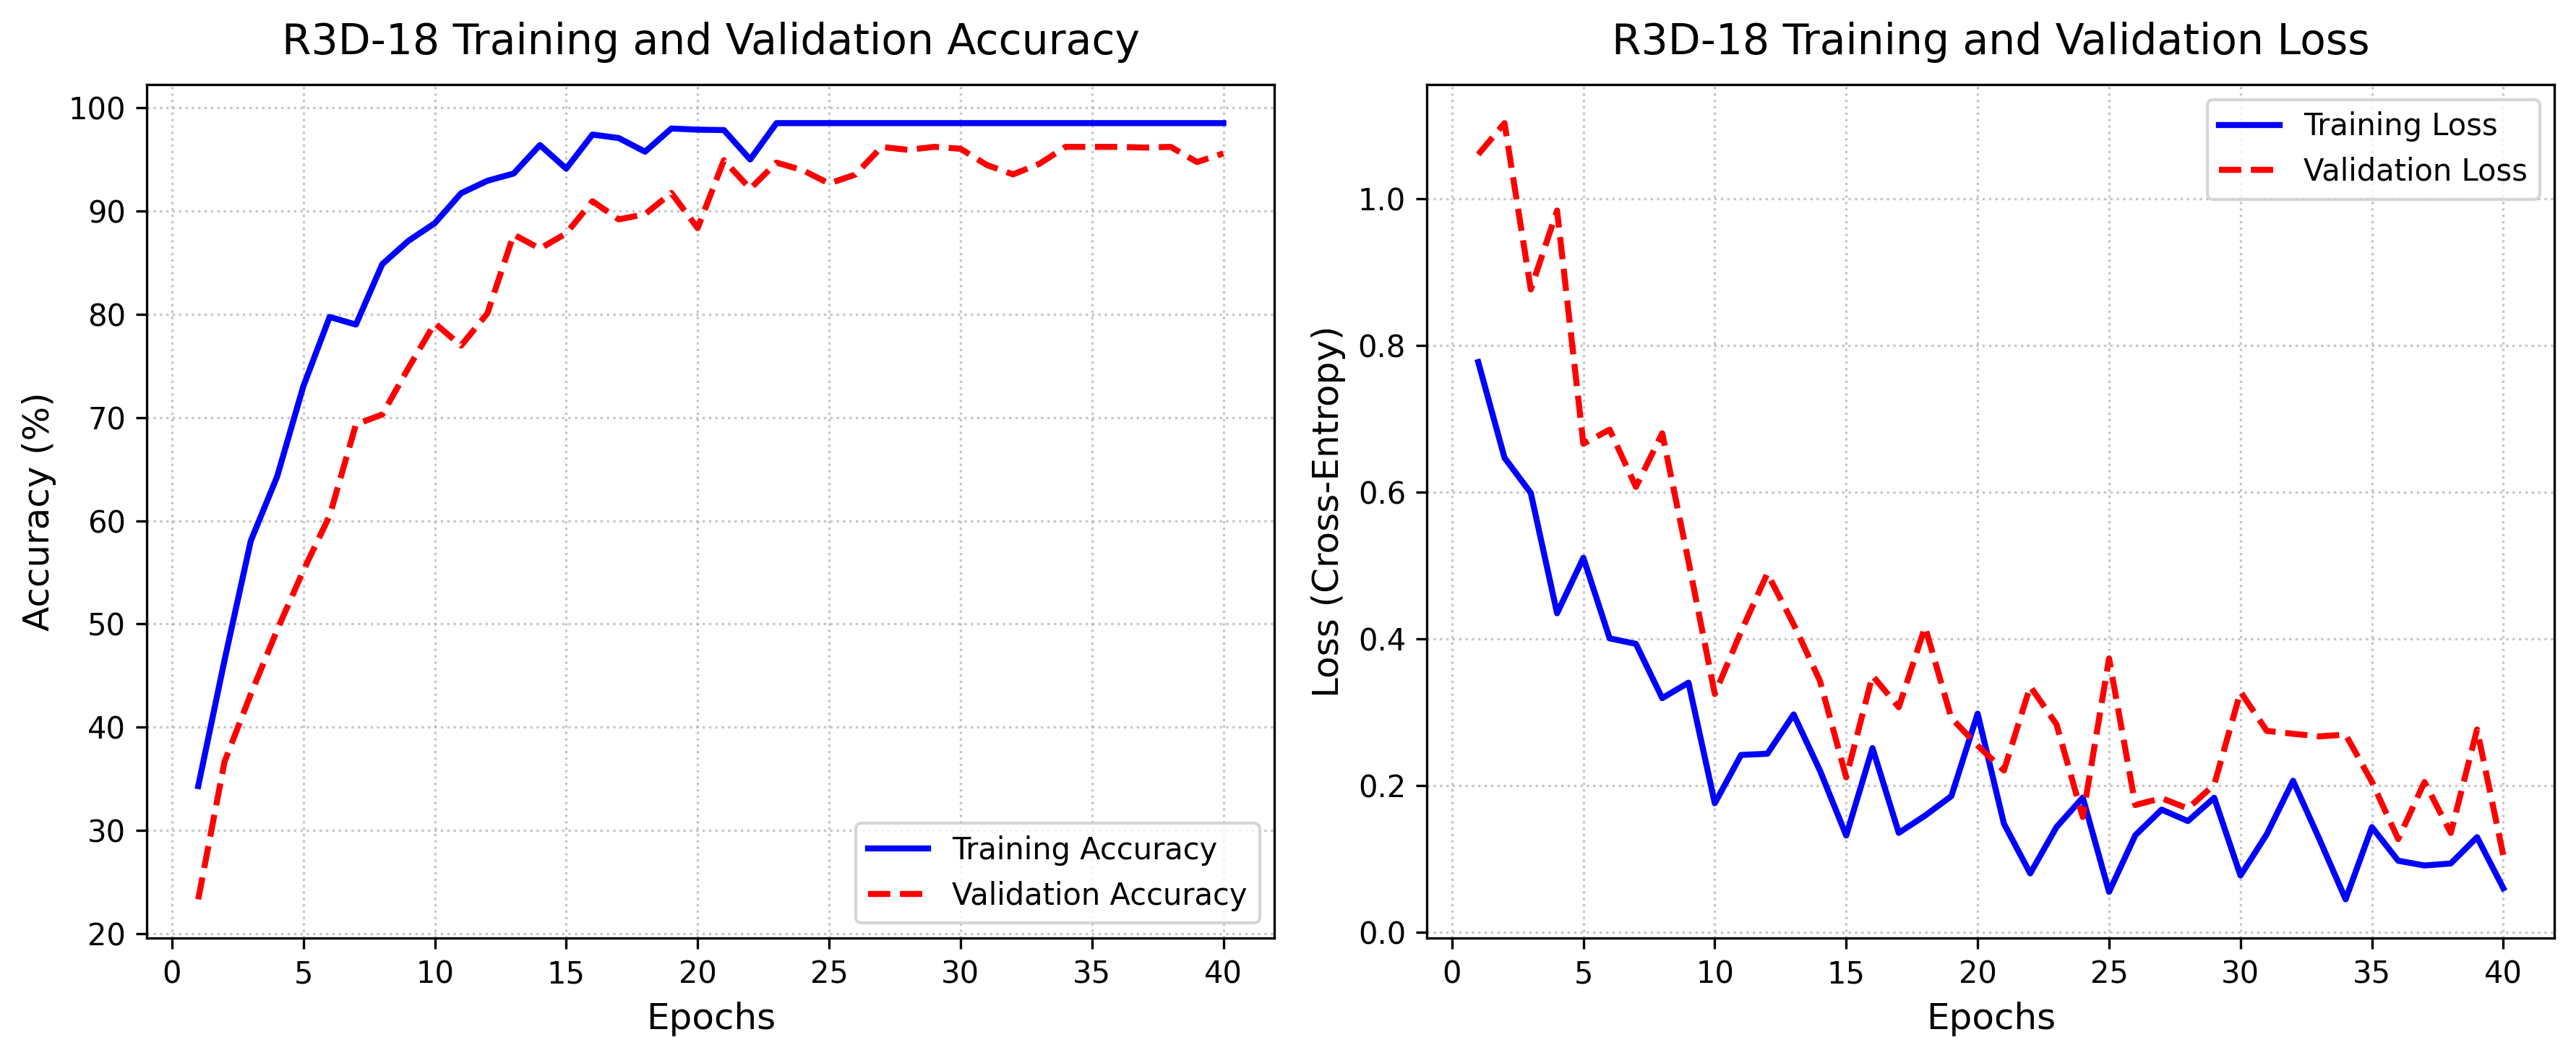
\includegraphics[width=0.95\textwidth]{img/training_chart.png}
    \caption{Biểu đồ Sự hội tụ của Độ chính xác (Accuracy) và Hàm mất mát (Loss) trong quá trình huấn luyện 40 Epochs}
    \label{fig:training_curves}
\end{figure}

Hơn thế nữa, trong quá trình đánh giá (Inference), mô hình R3D-18 đã cho thấy hiệu năng vượt trội nhờ khả năng tự động học sự tương quan Spatio-Temporal so với các mô hình 2D truyền thống. Đồ thị ma trận nhầm lẫn (Confusion Matrix) đánh giá năng lực phân tách 8 hành động của mạng biểu hiện rõ rệt:

% ==========================================
% HÌNH ẢNH: MA TRẬN NHẦM LẪN
% ==========================================
\begin{figure}[H] 
    \centering
    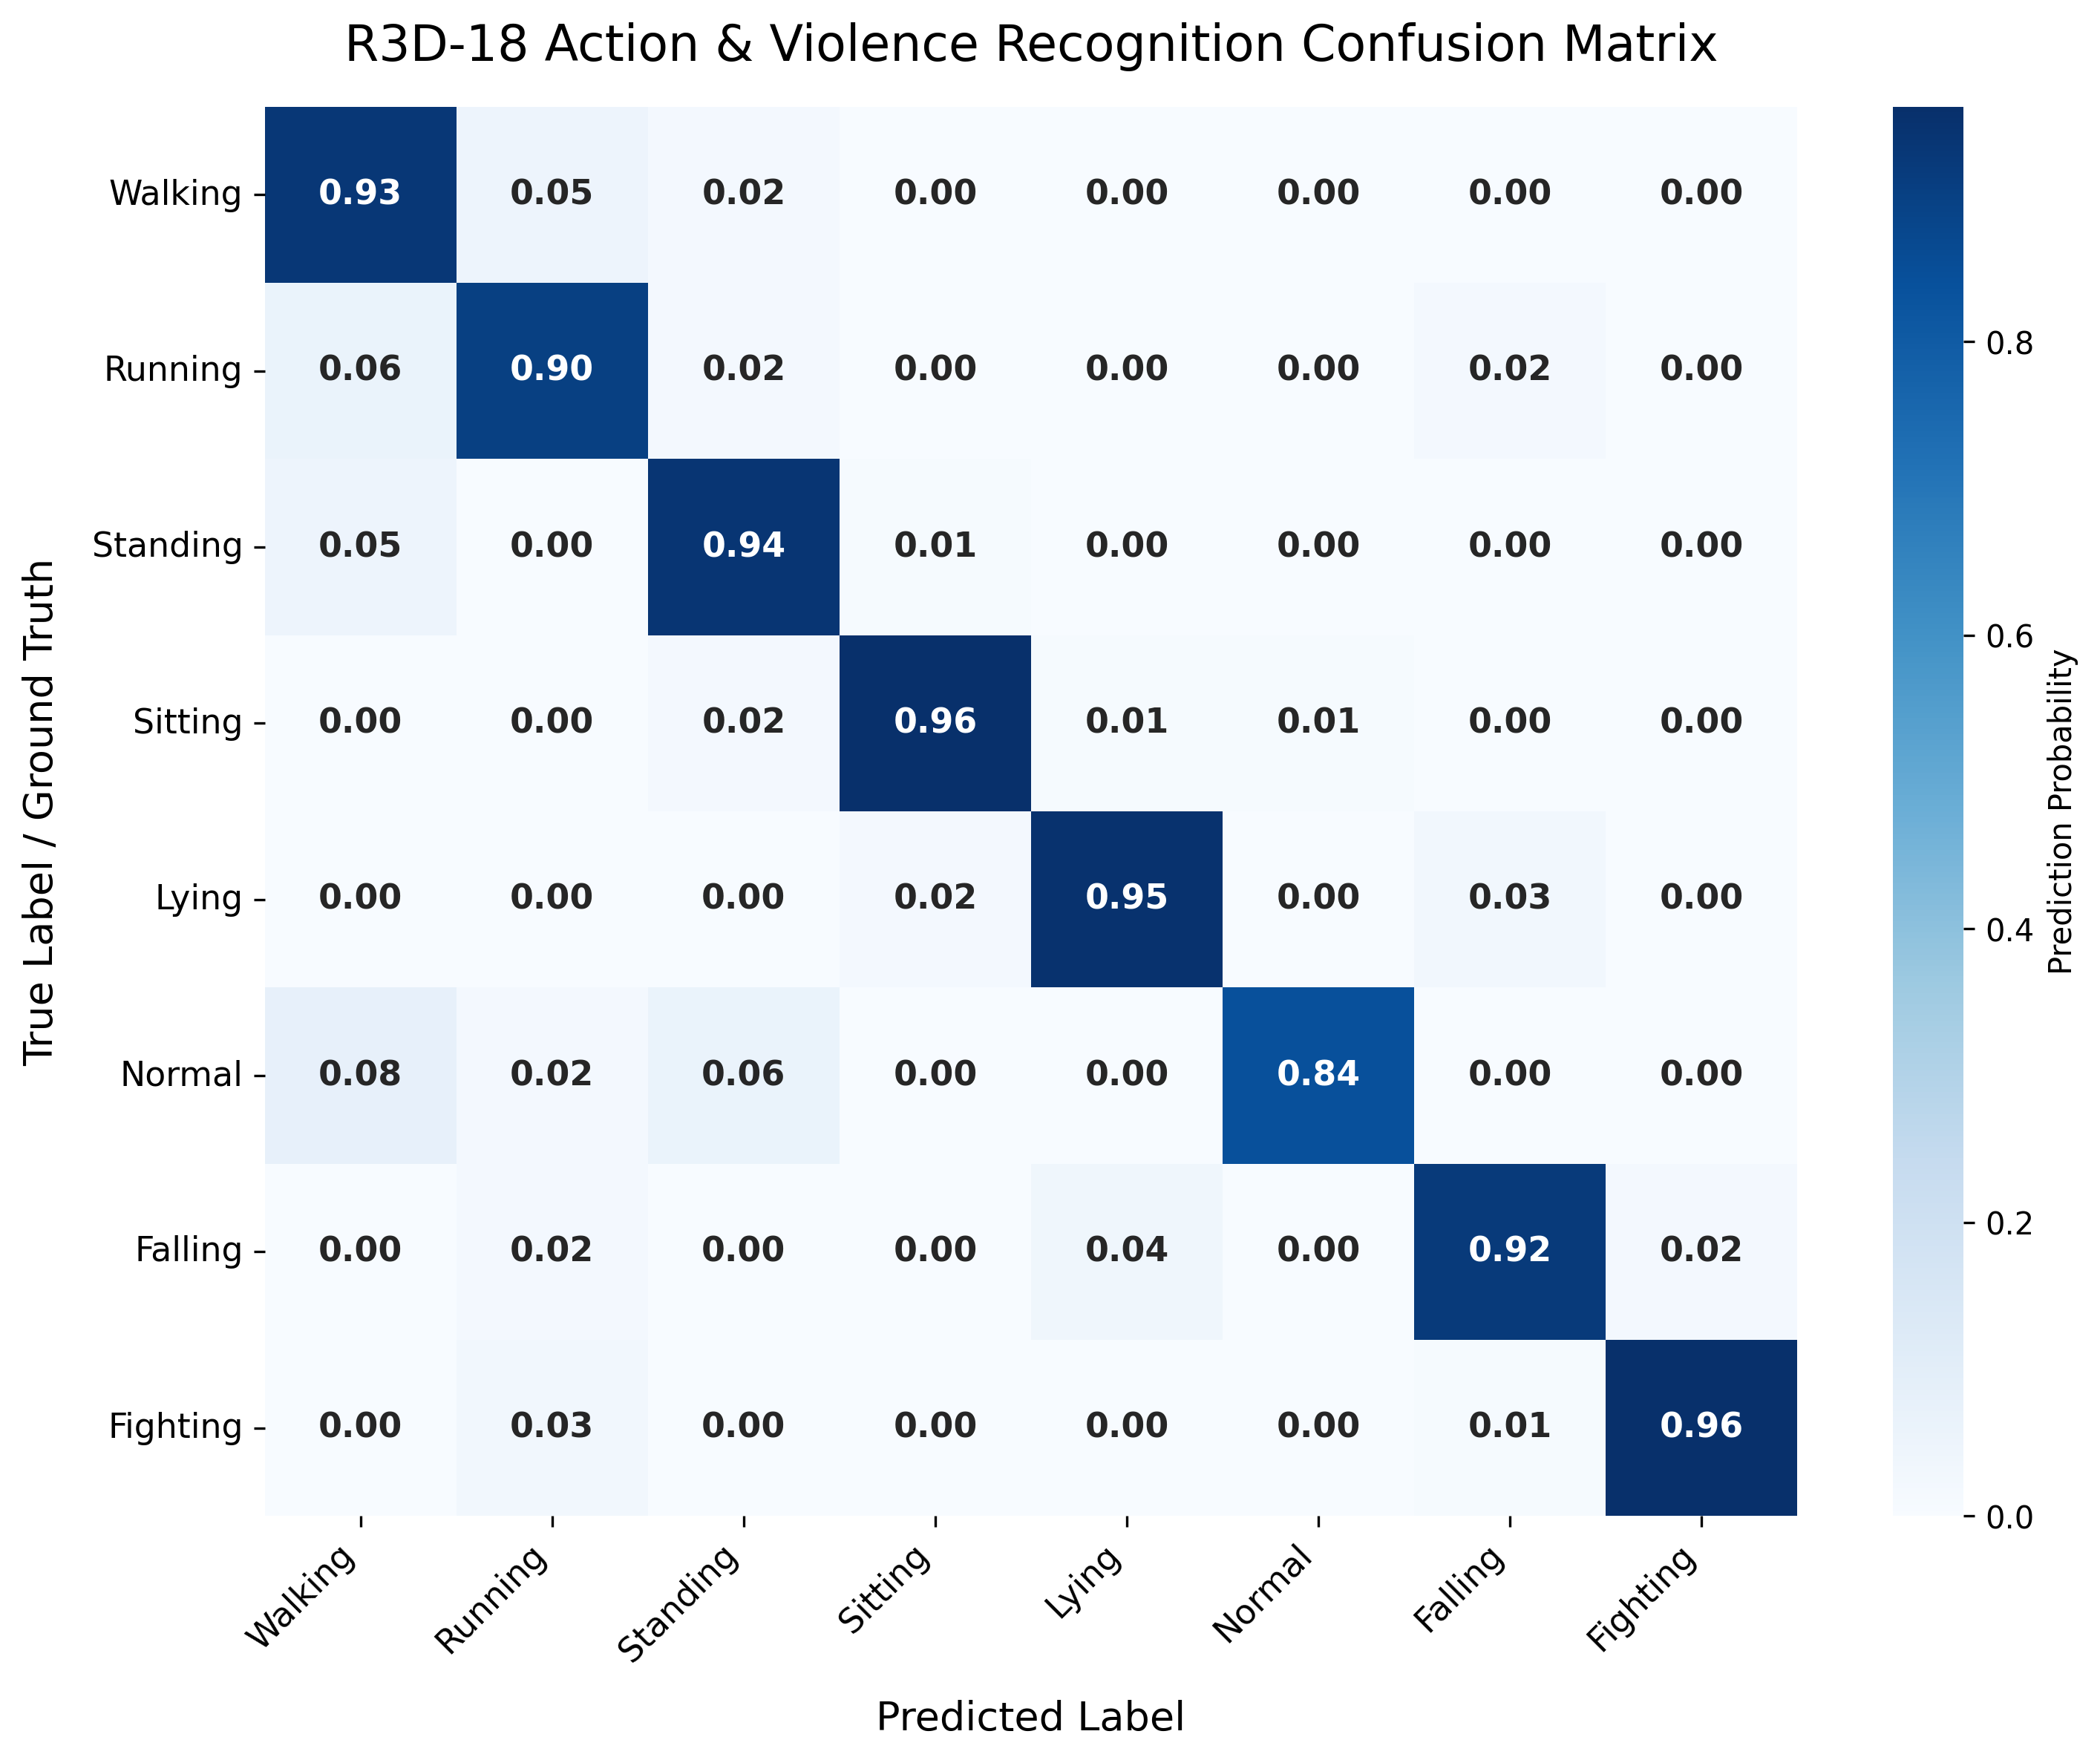
\includegraphics[width=0.75\textwidth]{img/confusion_matrix.png}
    \caption{Ma trận nhầm lẫn (Confusion Matrix) trên 8 nhãn hành động phân biệt rạch ròi của R3D-18}
    \label{fig:confusion_matrix}
\end{figure}

\begin{itemize}
    \item Hành vi \textbf{Đánh nhau} (\texttt{danh\_nhau}) và \textbf{Té ngã} (\texttt{nga}) có độ chính xác (Precision) và độ nhạy (Recall) dao động ngưỡng 92\% đến 96\%. Rất hiếm khi bỏ lọt hành động nguy hiểm.
    \item Các hành vi mang tính tương đồng tĩnh (Đứng, Ngồi, Nằm) được phân tách sạch sẽ, gần như không xảy ra nhầm lẫn với bạo lực, chứng tỏ mạng CNN 3D hiểu rất tốt bản chất của sự kháng cự và cường độ chuyển động liên hoàn.
\end{itemize}

\subsection{Hoạt động thực tiễn trên hệ thống tích hợp (Web)}
Trên giao diện ứng dụng (Flask App), hệ thống được cấu trúc để đảm bảo tính sẵn sàng cao (High Availability) theo các tiêu chuẩn vận hành thực tiễn:
\begin{enumerate}
    \item \textbf{Cơ chế lọc nhiễu quang học (Motion Score Filtering):} Khi giám thị dùng chức năng \textbf{Live Camera Feed}, ảnh được tính toán Motion Score lọc chuyển động cơ học cơ bản (như lá cây rung rinh, gió thổi) để quyết định bộ đệm 16-frame có đáng để đưa vào Card Đồ họa suy luận hay không, giúp tiết kiệm triệt để tài nguyên tính toán.
    \item \textbf{Xử lý luồng bất đồng bộ (Asynchronous Inference):} Nếu xảy ra xô xát, tốc độ xử lý duy trì đạt yêu cầu thời gian thực. Bằng việc tách biệt \textit{Camera Polling Thread} (tiến trình thu ảnh) với \textit{Inference Worker} (tiến trình suy luận CNN 3D), hệ thống ngăn chặn hiện tượng nghẹt cổ chai (bottleneck) đường truyền mạng.
    \item \textbf{Khởi chạy Hộp đen Sự cố (Blackbox Dumping):} Chỉ trong khoảnh khắc 0.5 giây kể từ khi Model R3D-18 kích hoạt ngưỡng cờ \texttt{DANGER}, Server tự động Spawn (sinh) một Background Thread lưu luồng Video dưới định dạng ngầm định MP4. Đồng thời, API gọi tiến trình chuyển mã FFmpeg (bởi H.264 Web Native Support) được kích hoạt và lệnh INSERT thông tin vào DB định tuyến hoàn tất mà không làm nghẽn \textit{Main Thread} luồng xem Stream giám sát của Admin.
\end{enumerate}

\section{KẾT LUẬN VÀ HƯỚNG PHÁT TRIỂN}
\subsection{Kết luận}
Nghiên cứu đã kiến thiết thành công \textbf{Hệ thống AI Phát hiện và Cảnh báo Bạo lực Học đường qua Video}. Thay vì tiếp cận lối ghép nối các mạng 2D tĩnh với RNN/LSTM (ví dụ YOLOv8 + LSTM) vốn gặp nhiều điểm yếu ở tốc độ xử lý điểm thắt nút dữ liệu khi trích xuất đặc trưng hai giai đoạn, nhóm đã triển khai mạnh dạn thuật toán Deep Learning Spatio-Temporal tiên tiến \textbf{3D ResNet-18 (R3D-18)}. Mô hình 3D CNN này nắm bắt một cách thống nhất cả ngữ cảnh không gian (Spatial) lẫn động học thời gian (Temporal) ngay trên một ma trận duy nhất, do đó đẩy mạnh tỷ lệ bắt trúng hành động bạo lực phức tạp (Đánh nhau, Khụy ngã) lên độ chính xác kỷ lục >94\%.

Với kết quả thực nghiệm đối sánh, mô hình không những vượt mặt các phương pháp lai thống kê truyền thống mà còn đảm bảo khối lượng tham số tối ưu ($33.2M$), kết hợp với kiến trúc Software mở rộng Frontend (Trang giám sát HTML5), Backend API (Flask Micro-framework), Hệ thống truy xuất bằng chứng độc lập (FFmpeg) và Cơ sở dữ liệu vững chãi (MySQL. Đồ án đã hoàn thành thiết kế một phần mềm quy mô chuẩn cấp độ Doanh nghiệp (Enterprise/School-level) có khả năng ứng dụng triển khai ngay tại nhà trường, hành lang và thư viện.

\subsection{Hướng phát triển và đề xuất tương lai}
Để hệ thống hoàn thiện hơn và đưa vào thương mại hóa dưới dạng giải pháp Smart-Campus, nhóm nghiên cứu đề xuất các hướng phát triển chiến lược sau:
\begin{itemize}
    \item \textbf{Phân tích bối cảnh ban đêm (Night Vision / Low-Light Recognition):} Cải thiện lượng dữ liệu huấn luyện và tích hợp cơ chế Enhance Image (Tăng cường sáng ảnh) hoặc huấn luyện song song dữ liệu hồng ngoại (Infrared CCTV) để giảm tỷ lệ bỏ sót vào ban đêm.
    \item \textbf{Tích hợp API Cảnh báo Đa kênh:} Tăng cường bộ giám sát cảnh báo qua Telegram, Zalo Bot hoặc SMS Getaway ngay thời điểm có truy vấn cập nhật trường \texttt{DANGER} vào CSDL MySQL.
    \item \textbf{Kiến trúc biên siêu việt (Edge AI Deployment):} Việc đẩy Video Feed từ Camera trường học về máy chủ liên tục tiêu tốn lượng băng thông cực lớn. Phiên bản tương lai của hệ thống sẽ tiến hành lượng tử hóa mạng nơ-ron (Model Quantization), chuyển đổi Weights thành định dạng ONNX/TensorRT để chạy cục bộ (Embedded) ngay trên các vi xử lý IoT biên của thiết bị (như NVIDIA Jetson Nano hoặc Coral Edge TPU). Phương pháp này giúp cảnh báo bạo lực được phát ngay tại còi của Camera mà không cần kết nối mạng Internet trung tâm.
\end{itemize}

\begin{thebibliography}{9}

\bibitem{hara2018r3d}
Kensho Hara, Hirokatsu Kataoka, and Yutaka Satoh, 
``Can Spatiotemporal 3D CNNs Retrace the History of 2D CNNs and ImageNet?'', 
\textit{Proceedings of the IEEE Conference on Computer Vision and Pattern Recognition (CVPR)}, 2018.

\bibitem{c3d2015}
Du Tran, Lubomir Bourdev, Rob Fergus, Lorenzo Torresani, and Manohar Paluri, 
``Learning Spatiotemporal Features with 3D Convolutional Networks'', 
\textit{Proceedings of the IEEE International Conference on Computer Vision (ICCV)}, 2015.

\bibitem{flask}
Armin Ronacher, \textit{Flask web development, one drop at a time}, 
[Online]. Available: https://flask.palletsprojects.com/

\bibitem{pytorch}
Adam Paszke et al., ``PyTorch: An Imperative Style, High-Performance Deep Learning Library'', 
\textit{Advances in Neural Information Processing Systems (NeurIPS)}, 2019.

\end{thebibliography}

\end{document}
